\documentclass[t,english]{beamer}
\usepackage{multicol}
\usepackage{tikz}
\usepackage{grscolors}

\usetheme{GRS}

\title[]{Unstructured FEM:\\ 2D Unsteady Heat Diffusion}
\author{Abhishek Y. Deshmukh, Raghavan Lakshmanan, \\Mohsin Ali Chaudry, A. Emre Ongut}
\date{January 31, 2014}

%
% Templates to change
%
%\setbeamertemplate{stock photo left}[default][grs-stock1]
%\setbeamertemplate{stock photo middle}[default][grs-stock2]
%\setbeamertemplate{stock photo right}[default][grs-stock3]


\AtBeginSection{
\begin{frame}{Contents}
	\begin{multicols}{2}
     \tableofcontents[currentsection,hidesubsections]
	\end{multicols}
\end{frame}
}

\begin{document}

\maketitle

%============================================================

\section{Objective}

\begin{frame}[c]{Objective}
\begin{itemize}
\item To develop a parallel finite element solver that uses unstructured grid to solve a 2D transient heat diffusion problem.

\item Application to a realistic engineering heat transfer problem, Heat diffusion in Microchannels in the heat sink of microprocessors.
\end{itemize}

\end{frame}

\section{Finite Element Method}

\begin{frame}[c]{General Steps}

\begin{enumerate}
\item Preprocessing
	\begin{itemize}
	\item Define a domain of interest
	\item Discretization of domain into finite elements 
	\end{itemize}
\item Solution
	\begin{itemize}
	\item Define shape functions to represent the behaviour of elements
	\item Construct local stiffness matrix and then ultimately global stiffness matrix
	\item Apply boundary condition, initial conditions and forcing function
	\item Solving linear system of algebraic equations
	\end{itemize}
\item Postprocessing
	\begin{itemize}
	\item Analyse the solution
	\end{itemize}
\end{enumerate}
\end{frame}

\section{FEM Formulation}
\begin{frame}{2D Unsteady Heat Diffusion Equation}
$$\frac{\partial T}{\partial t}-\alpha \nabla^2T =f , \text{in }  \Omega \in \Re^2 $$ 
where $\alpha$ is diffusion coefficient.
$$ \alpha = \frac{k}{\rho c_p}$$
k is heat conductivity, $\rho$ is the density and $c_p$  is the specific heat capacity of the material.
$$ f = \frac{\dot{q}}{\rho c_p}$$
where $\dot{q}$ is heat generation per unit volume.
\end{frame}

\begin{frame}{Initial and Boundary Conditions}
\begin{itemize}
\item Intial condition:
	$T(x,y,0) = T_0(x,y)$
\item Boundary conditions
	\begin{itemize}
	\item Dirichlet:
	 \\
		$T(x,0,t) = T_1$, $T(x,L,t) = T_2$, $T(0,y,t) = T_3$, $T(L,y,t) = T_4$
	\\
	\item Neumann:
	\\
$k\left(n_x\frac{\partial T}{\partial x} + n_y\frac{\partial T}{\partial y}\right) = q_0$
	\\
	\item Robin (Mixed):
	
	$h(T-T_{\inf}) = -k\left(n_x\frac{\partial T}{\partial x} + n_y\frac{\partial T}{\partial y}\right)$
	\end{itemize}
\end{itemize}
\end{frame}

\begin{frame}[c]{Weighted Residual Method}
$$\int_\Omega (w \frac{\partial T}{\partial t}  +\alpha w\nabla^2T)d\Omega= \int_\Omega wfd\Omega $$
 
where w is a weigthing function or test function.

Integrating by parts,
 $$\int_\Omega (w \frac{\partial T}{\partial t}  +\alpha \nabla w .\nabla T)d\Omega = \int_\Omega wfd\Omega + \frac{1}{\rho c_p}\int_ \Gamma w\underbrace{(k \hat{n}.\nabla T)}_{k(n_x\frac{\partial T}{\partial x} + n_y\frac{\partial T}{\partial y})}d\Gamma $$
\end{frame}

\begin{frame}[c]{Approximation}
\begin{itemize}

\item Approximate the temperature as a piecewise linear combination of shape functions $S_j(x,y)$. 
\item These shape functions remain constant over time. The coefficients $T_j(t)$ are time dependent.

 $${ T }(x,y,t)=\sum _{ j=1 }^{ nn }{ { T }_{ j }(t){ S }_{ j }(x,y) } $$

\item Galerkin Finite Element Method: $$w=S_i(x)$$
\end{itemize}
\end{frame}

\begin{frame}[c]{Approximation [contd.]}
$$\underbrace{\sum_{j=1}^{nn} \int_\Omega (S_i S_j)d\Omega \frac{\partial T_j}{\partial t}}_{[M][\dot{T}]} - \underbrace{\sum_{j=1}^{nn}[\int_\Omega \alpha (\frac{\partial S_i}{\partial x}\frac{\partial S_j}{\partial x} + \frac{\partial S_i}{\partial y}\frac{\partial S_j}{\partial y})d\Omega] T_j }_{[K][T]}$$ $$= \underbrace{\int_\Omega S_i	f d\Omega}_{[F]}  +  \underbrace{\frac{1}{\rho c_p} \int_\Gamma S_i (k \hat{n}.\nabla T) d\Gamma}_{[B]}$$
$i,j = 1,2,...,nn	 $
$$[K]_{ij} = \int_\Omega \alpha (\frac{\partial S_i}{\partial x}\frac{\partial S_j}{\partial x} + \frac{\partial S_i}{\partial y}\frac{\partial S_j}{\partial y})d\Omega$$
\end{frame}

\begin{frame}[c]{Triangular Elements}
\begin{figure}
\centering
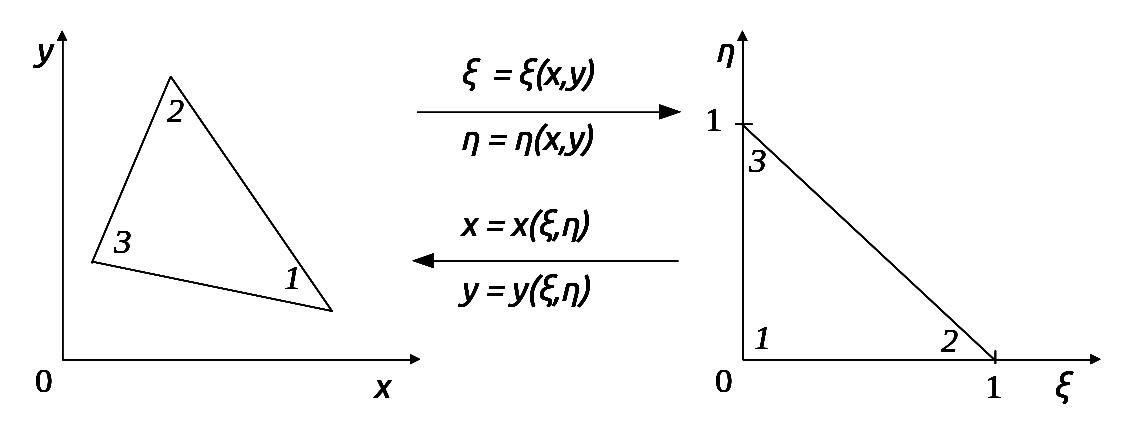
\includegraphics[scale=0.2]{master_elem.png}

Co-ordinate transformation
\end{figure}
Shape functions:

$S_1(\xi,\eta) = 1 - \xi - \eta$,  $S_2(\xi,\eta) = \xi$, $S_3(\xi,\eta) = \eta$
\end{frame}

\begin{frame}
$$\frac{\partial S_1}{\partial \xi} = -1  ,    \frac{\partial S_2}{\partial \xi} = 1 ,   \frac{\partial S_3}{\partial \xi} = 0,   \frac{\partial S_1}{\partial \eta} = -1,    \frac{\partial S_2}{\partial \eta} = 0,     \frac{\partial S_3}{\partial \eta} = 1$$

$$\frac{\partial S_i}{\partial \xi} = \frac{\partial S_i}{\partial x}\frac{\partial x}{\partial \xi} + \frac{\partial S_i}{\partial y}\frac{\partial y}{\partial \xi}, \frac{\partial S_i}{\partial \eta} = \frac{\partial S_i}{\partial x}\frac{\partial x}{\partial \eta} + \frac{\partial S_i}{\partial y}\frac{\partial y}{\partial \eta}$$

$$\begin{bmatrix}
\frac{\partial S_i}{\partial \xi} \\ \\ \frac{\partial S_i}{\partial \eta}
\end{bmatrix} = \underbrace{\begin{bmatrix}
\frac{\partial x}{\partial \xi} \quad \frac{\partial y}{\partial \xi}\\ \\ \frac{\partial x}{\partial \eta} \quad \frac{\partial y}{\partial \eta} 
\end{bmatrix}}_{Jacobian} \begin{bmatrix}
\frac{\partial S_i}{\partial x} \\ \\ \frac{\partial S_i}{\partial y}
\end{bmatrix}$$
\end{frame}

\begin{frame}
Isoparametric formulation:
$x(\xi,\eta) = \sum_{j=1}^{nen} x_j^e S_j(\xi,\eta) \text{ , }
 y(\xi,\eta) = \sum_{j=1}^{nen} y_j^e S_j(\xi,\eta)$
 Jacobian:
 $$\begin{bmatrix}J\end{bmatrix} = \begin{bmatrix}
\frac{\partial S_1}{\partial \xi} \quad \frac{\partial S_2}{\partial \xi}\quad \frac{\partial S_3}{\partial \xi}\\ \\ \frac{\partial S_1}{\partial \eta} \quad \frac{\partial S_2}{\partial \eta}\quad \frac{\partial S_3}{\partial \eta} 
\end{bmatrix} \begin{bmatrix}
x_1^e \quad y_1^e\\ \\ x_2^e \quad y_2^e \\ \\ x_3^e \quad y_3^e\end{bmatrix} = \begin{bmatrix}
\frac{\partial x}{\partial \xi} \quad \frac{\partial y}{\partial \xi}\\ \\ \frac{\partial x}{\partial \eta} \quad \frac{\partial y}{\partial \eta} 
\end{bmatrix}$$
But we need $[J]^{-1}$ which is the inverse mapping. 
$$\begin{bmatrix}
\frac{\partial S_i}{\partial x} \\ \\ \frac{\partial S_i}{\partial y}
\end{bmatrix} = \underbrace{\begin{bmatrix}
\frac{\partial \xi}{\partial x} \quad \frac{\partial \eta}{\partial x}\\ \\ \frac{\partial \xi}{\partial y} \quad \frac{\partial \eta}{\partial y} 
\end{bmatrix}}_{[J]^{-1}}\underbrace{\begin{bmatrix}
\frac{\partial S_i}{\partial \xi} \\ \\ \frac{\partial S_i}{\partial \eta}
\end{bmatrix}}_{known} $$
\end{frame}

\begin{frame}
Calculation of element level stiffness matix:
$$K_{ij}^e = \int_{\Omega_e} \alpha (\frac{\partial S_i}{\partial x}\frac{\partial S_j}{\partial x} + \frac{\partial S_i}{\partial y}\frac{\partial S_j}{\partial y})dx dy \text{     i,j = 1,2,...,nen}$$
Integral transformation to master element:
$$K_{ij}^e = \int_{0}^1 \int_0^{1-\xi} \alpha [f_k(\xi,\eta)]|J|d\xi d\eta$$

$$ f_k(\xi,\eta) = \left(\frac{\partial S_i}{\partial \xi}\frac{\partial \xi}{\partial x} + \frac{\partial S_i}{\partial \eta}\frac{\partial \eta}{\partial x}\right)\left(\frac{\partial S_j}{\partial \xi}\frac{\partial \xi}{\partial x} + \frac{\partial S_j}{\partial \eta}\frac{\partial \eta}{\partial x}\right)$$
$$+ \left(\frac{\partial S_i}{\partial \xi}\frac{\partial \xi}{\partial y} + \frac{\partial S_i}{\partial \eta}\frac{\partial \eta}{\partial y}\right)\left(\frac{\partial S_j}{\partial \xi}\frac{\partial \xi}{\partial y} + \frac{\partial S_j}{\partial \eta}\frac{\partial \eta}{\partial y}\right)$$
$i,j = 1,2,...,nen$
\end{frame}

\begin{frame}
Numerical Integration using 7 point Gauss Quadrature rule:
\begin{figure}[ht!]
\centering
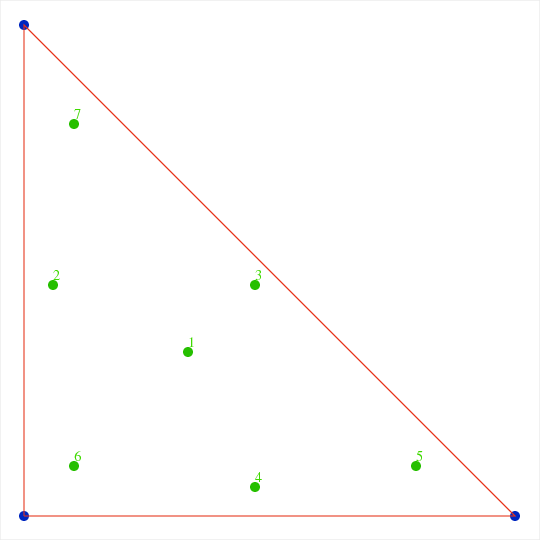
\includegraphics[width=40mm]{GQP7.png}
\end{figure}
$$K_{ij}^e \simeq \sum_{l=1}^{nGQP}f_k(\xi_l,\eta_l) w_l$$
\end{frame}

\begin{frame}[c]{Solution}
In matrix form :
$[M][\dot{T}]+[K][T]=[F]+[B]$
\\
Forward Euler explicit differencing in time:

$$ \frac{dT}{dt } \mid_s = \frac{T^{s+1}-T^s}{ \Delta t} +O( \Delta t)$$

$$[M]  \frac{[T]^{s+1}-[T]^s}{ \Delta t} +[K][T]^s=[F]+[B]$$

$$[M] [T]^{s+1}=[M][T]^s+{ \Delta t} ([F]+[B]-[K][T]^s)$$
$$[M] [T]^{s+1}=[RHS]^s$$

\end{frame}

\begin{frame}{Lumping of Mass Matrix}

The inversion of Mass matrix can be avoided if we do a physical approximation called lumping of mass matrix.

Consistent element  mass matrix: $[M_{cij}]$

Lumped element mass matrix: $[M_{Lij}]$

$${ M }_{ Lii }={ M }_{ cii }\frac { \sum _{ i=1 }^{ n }{ \sum _{ j=1 }^{ n }{ { M }_{ cij } }  }  }{ \sum _{ j=1 }^{ n }{ { M }_{ cjj } }  }$$	  

This is correct only for linear elements.

$[M_{Lij}]$ is a diagonal matrix.
\end{frame}

\begin{frame}{Boundary Integral}
\begin{itemize}
\item Dirichlet: $[B]_{j} = T_w$, $[K]_{jj} = 1$, $[K]_{ij} = 0$ $\forall i\neq j$

For example, if for some element, node temperatures T1 and T3 are known then [B] and [K] for that element can be written as:
$$[B] = \begin{bmatrix}
T_w \\
B_2 \\
T_w
\end{bmatrix} \text{  and  } [K] = \begin{bmatrix}
1 \quad 0 \quad 0 \\
\ast \quad \ast \quad \ast \\
0 \quad 0 \quad 1
\end{bmatrix} $$

$\ast$ indicate non-zero values.
\end{itemize}
\end{frame}

\begin{frame}{Boundary Integral [contd.]}
\begin{itemize}
\item Neumann (Flux Variable(FV) = $q_{in}$):\begin{figure}[ht!]
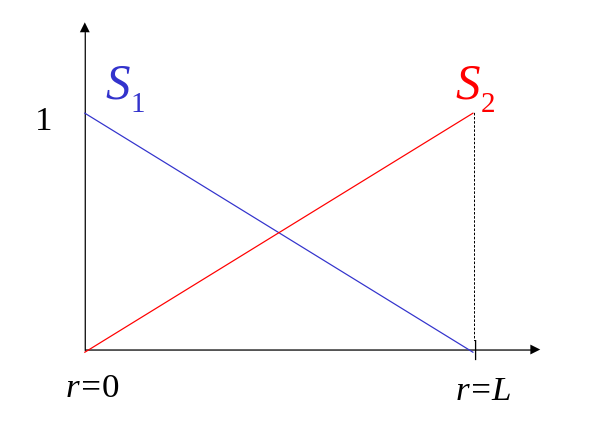
\includegraphics[trim=-1200 0 0 450,scale=0.15]{edge_shape_fun.png}
\end{figure}
$$B_1^e = \frac{1}{\rho c_p} \int_\Gamma S_1 (FV)d\Gamma = \frac{1}{\rho c_p}\int_0^L (1-\frac{r}{L}) q_{in}dr = \frac{q_{in} L}{2 \rho c_p} $$
$$B_2^e = \frac{1}{\rho c_p} \int_\Gamma S_2 (FV)d\Gamma = \frac{1}{\rho c_p} \int_0^L \frac{r}{L} q_{in}dr = \frac{q_{in} L}{2 \rho c_p} $$

$$[B] = \begin{bmatrix}
\frac{q_{in}L}{2 \rho c_p} \\
\frac{q_{in}L}{2 \rho c_p} \\
0
\end{bmatrix}$$ 
\end{itemize}
\end{frame}

\begin{frame}{Boundary Integral [contd.]}
\begin{itemize}
\item Robin(Mixed type):
Flux variable (FV) can be expressed as $$-k \hat{n}.\nabla T = h(T - T_{\infty})$$
$FV = a PV + b$ where a = -h and b = $hT_{\infty}$

$$B_1^e = \frac{1}{\rho c_p} \int_\Gamma S_1 (FV)d\Gamma = \frac{1}{\rho c_p} \int_0^L (1-\frac{r}{L}) (a PV + b)dr$$
$$B_2^e = \frac{1}{\rho c_p} \int_\Gamma S_2 (FV)d\Gamma = \frac{1}{\rho c_p} \int_0^L \frac{r}{L} (a PV + b)dr$$
Primary variable (PV) temperature: 
$$PV = S_1 T_1 + S_2 T_2$$
\end{itemize}
\end{frame}

\begin{frame}{Boundary Integral [contd.]}
$$B_1^e = \frac{1}{\rho c_p} \int_0^L (1-\frac{r}{L})[a ((1-\frac{r}{L})T_1 + \frac{r}{L}T_2 ) + b]dr$$ $$= \frac{L}{6 \rho c_p}(3b + 2aT_1 + aT_2)$$
$$B_2^e = \frac{1}{\rho c_p} \int_0^L \frac{r}{L}[a ((1-\frac{r}{L})T_1 + \frac{r}{L}T_2 ) + b]dr $$ $$= \frac{L}{6 \rho c_p}(3b + aT_1 + 2aT_2)$$
\end{frame}

\begin{frame}{Boundary Integral [contd.]}
Element boundary vector can be written as:
$$[B] = \begin{bmatrix}
\frac{L}{6 \rho c_p}(3b + 2aT_1 + aT_2) \\
\frac{L}{6 \rho c_p}(3b + aT_1 + 2aT_2) \\
0
\end{bmatrix}$$
 Coefficients of $T_1$ and $T_2$ transferrd to K. Modified [B] and corresponding [K] can be written as:
$$[B] = \begin{bmatrix}
\frac{Lb}{2 \rho c_p} \\
\frac{Lb}{2 \rho c_p} \\
0
\end{bmatrix} \text{  and  } [K] = \begin{bmatrix}
(\ast - \frac{aL}{3 \rho c_p}) \quad (\ast - \frac{aL}{6 \rho c_p}) \quad \quad \ast \\
(\ast - \frac{aL}{6 \rho c_p}) \quad (\ast - \frac{aL}{3 \rho c_p}) \quad \quad \ast \\
\ast \quad \quad \quad \quad \ast \quad \quad \quad \quad \ast
\end{bmatrix} $$
\end{frame}

\section{Implementation}

\begin{frame}[c]{Program Flow Chart}
\begin{multicols}{2}
\begin{itemize}
\item[1]Preprocessing Stage:
	\begin{itemize}
	\item Reading settings file
	\item Reading mesh data
	\end{itemize}
\item[2]Solution Stage:
	\begin{itemize}
	\item Calculating Jacobian matrix for all elements
	\item Calculating element stiffness matrix for all     elements
	\item Applying boundary conditions
	\item Explicit Solver
	\end{itemize}
\item[3] Post Processing Stage
\end{itemize}
\columnbreak
\begin{figure}[ht!]
\centering
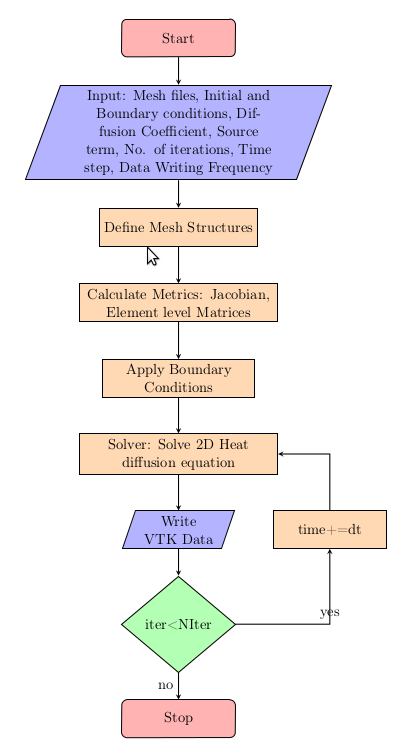
\includegraphics[trim=0 0 0 150,scale=0.4]{serialflowchart.png}
\end{figure}
\end{multicols}
\end{frame}

\section{Verification}
\begin{frame}[c]{Case 1: 1D}
A simple 1D case is taken as an example.
Domain: x $\in$ [0,L] L = 2.

Initial condition: $T_i = T(x,0) = 1000 K$
\\
Boundary Conditions: $T_L = T(0,t)) = 0$, 
$T_R = T(L,t)) = 0$, $T_{top}$ and $T_{bottom}$ are insulated
\\
Analytical Solution: $$T(x,t) = \sum_{n=1}^{\infty} B_n sin(\frac{n \pi x}{L}) e^{-\frac{n^2 \pi^2 \alpha t}{L^2}} $$ where $\alpha$ is diffusion coefficient and  $$B_n = -T_i \frac{2(-1 + (-1)^n)}{n\pi}$$

\end{frame}

\begin{frame}[c]{Comparison with Analytical solution}
\begin{figure}[ht!]
\centering
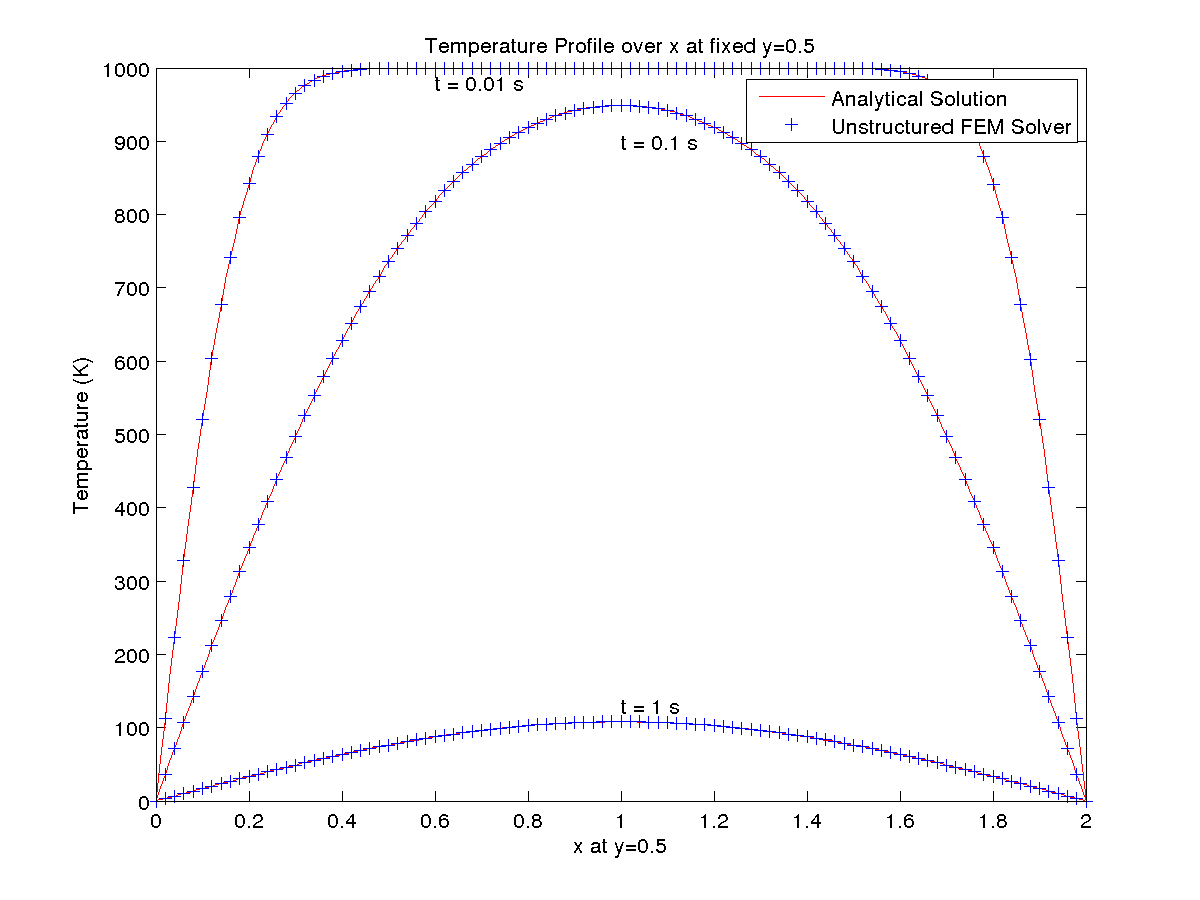
\includegraphics[scale=0.4]{1D.png}
\end{figure}
\end{frame}

\begin{frame}[c]{Case 2: 2D Quenching of a Billet\cite{jw}}

Domain: A long billet of rectangular cross section $2a \times 2b$ (a=2, b=1). Because of symmetry, analyze one quarter of the cross section 
\\
Shifted temperature: $\theta(x,y,t) = T(x,y,t) - T_{\infty}$

Material properties: $\alpha = 1$, $\rho = 1$, $c_p = 1$, $h = 1$

Initial condition: $\theta (x,y,0) = T_i - T_{\infty} = \theta_i$, $T_i = 1000$, $T_{\infty} = 300$
\\
Boundary Conditions: 
\begin{multicols}{2}
 $x = 0$:  $\frac{\partial \theta}{\partial x} = 0$\\$x = a$:  $\frac{\partial \theta}{\partial x} = -\frac{h}{k} \theta (a,y,t)$
 
\columnbreak
$y = 0$:  $\frac{\partial \theta}{\partial y} = 0$\\ $y = b$: $\frac{\partial \theta}{\partial y} = -\frac{h}{k} \theta (x,b,t)$
\end{multicols}
\end{frame}

\begin{frame}

Analytical solution:$$\frac{\theta}{\theta_i} = 4 \sum_{n=1}^{\infty} \sum_{m=1}^{\infty} e^{(-\alpha(\lambda_n^2 + \beta_m^2) t)}\times$$ $$ \frac{sin(\lambda_n a) cos(\lambda_n x) sin(\beta_m b) cos(\beta_m y)}{[\lambda_n a + sin(\lambda_n a)cos(\lambda_n a)][\beta_m b + sin(\beta_m b)cos(\beta_m b)]} $$ where $\alpha$ is diffusion coefficient and  the eigenvalues $\lambda_n$ and $\beta_m$ are the roots of trancendental equations.
\begin{multicols}{2}
$$\lambda_n tan(\lambda_n a) = \frac{h}{k}$$

\columnbreak
$$\beta_m tan(\beta_m b) = \frac{h}{k}$$
\end{multicols}
 where k is conductivity of the billet matrial.
\end{frame}

\begin{frame}[c]{Results}
\begin{figure}[ht!]
\centering
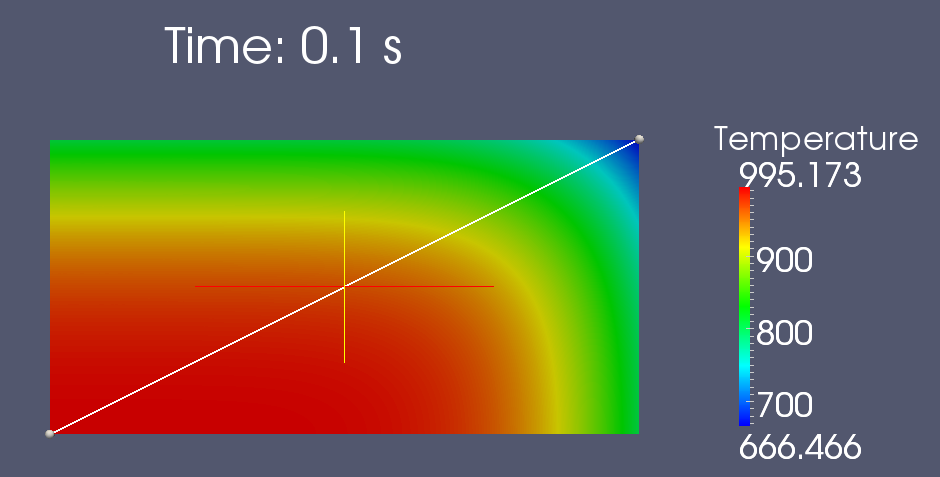
\includegraphics[scale=0.4]{billet_paraview.png}
\end{figure}
\end{frame}

\begin{frame}[c]{Results [contd.]}
\begin{multicols}{2}
\begin{figure}[ht!]
\centering
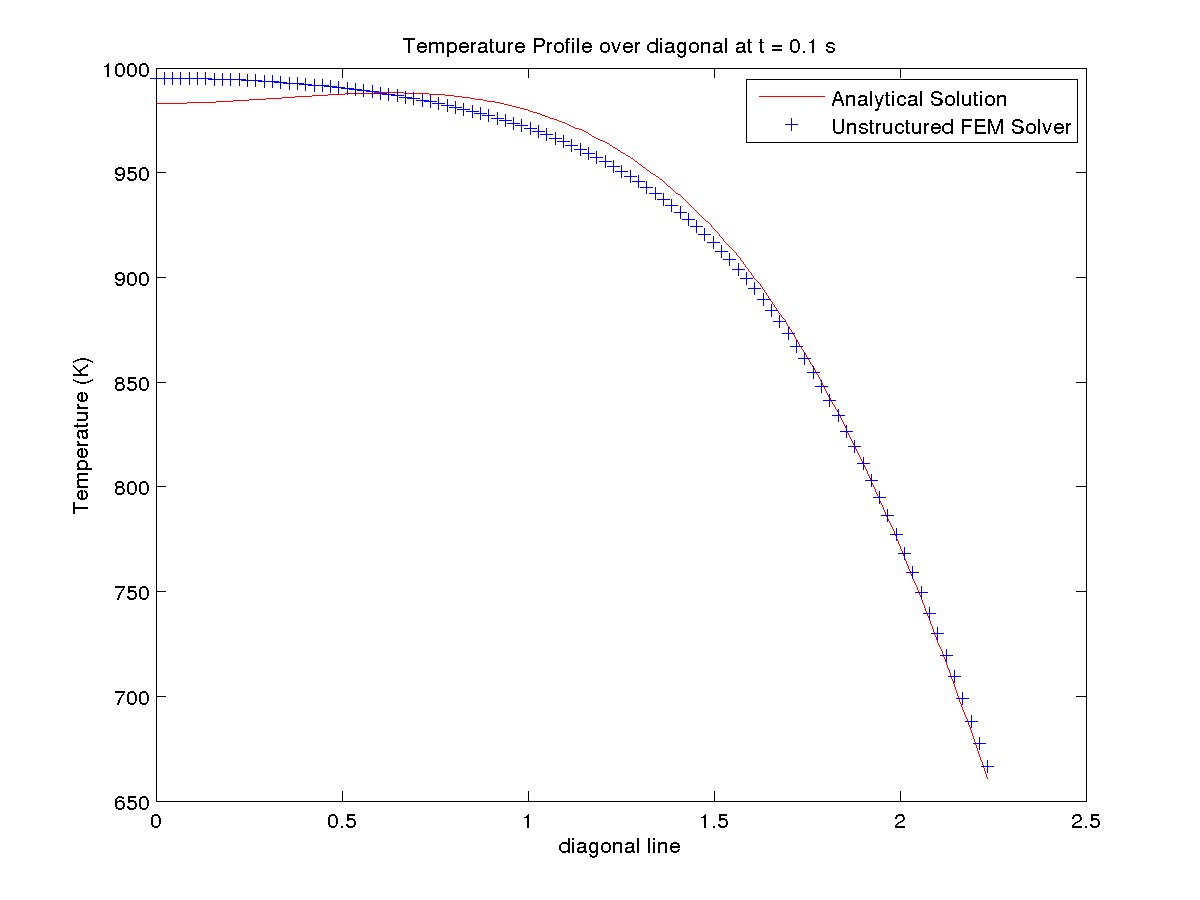
\includegraphics[trim=100 0 0 50,scale=0.31]{billet01.png}
\end{figure}

\columnbreak

\begin{figure}[ht!]
\centering
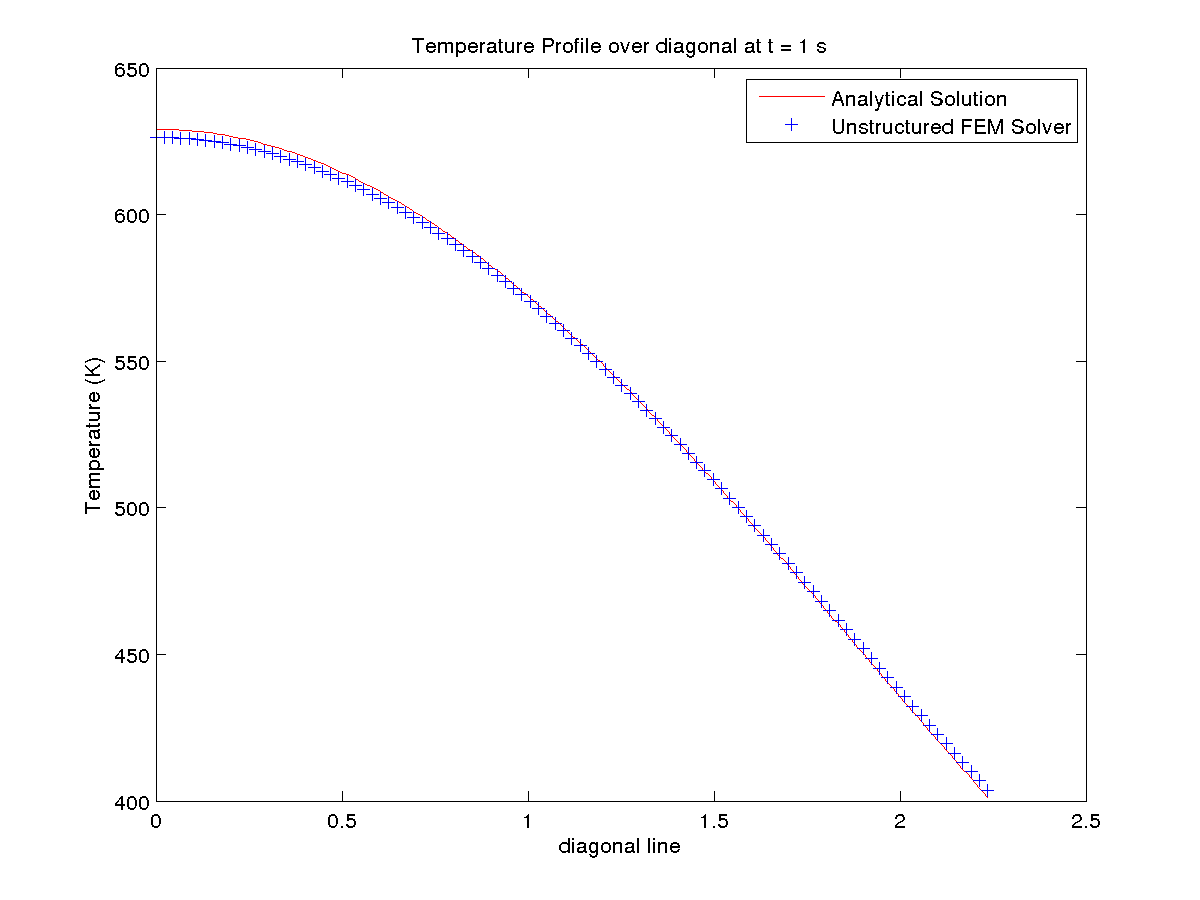
\includegraphics[trim=50 0 0 50,scale=0.31]{billet1.png}
\end{figure}
\end{multicols}
\end{frame}

\section{Optimization}
\begin{frame}{Optimization}
\begin{multicols}{2}
\begin{itemize}
\item Manual Optimization
	\begin{itemize}
	\item Local arrays and variables
	\item Loop unrolling
	\end{itemize}
\item Automatic Optimization
	\begin{itemize}
	\item O1
	\item O2
	\item O3
	\end{itemize}
\end{itemize}

\columnbreak
\begin{figure}[ht!]
\centering
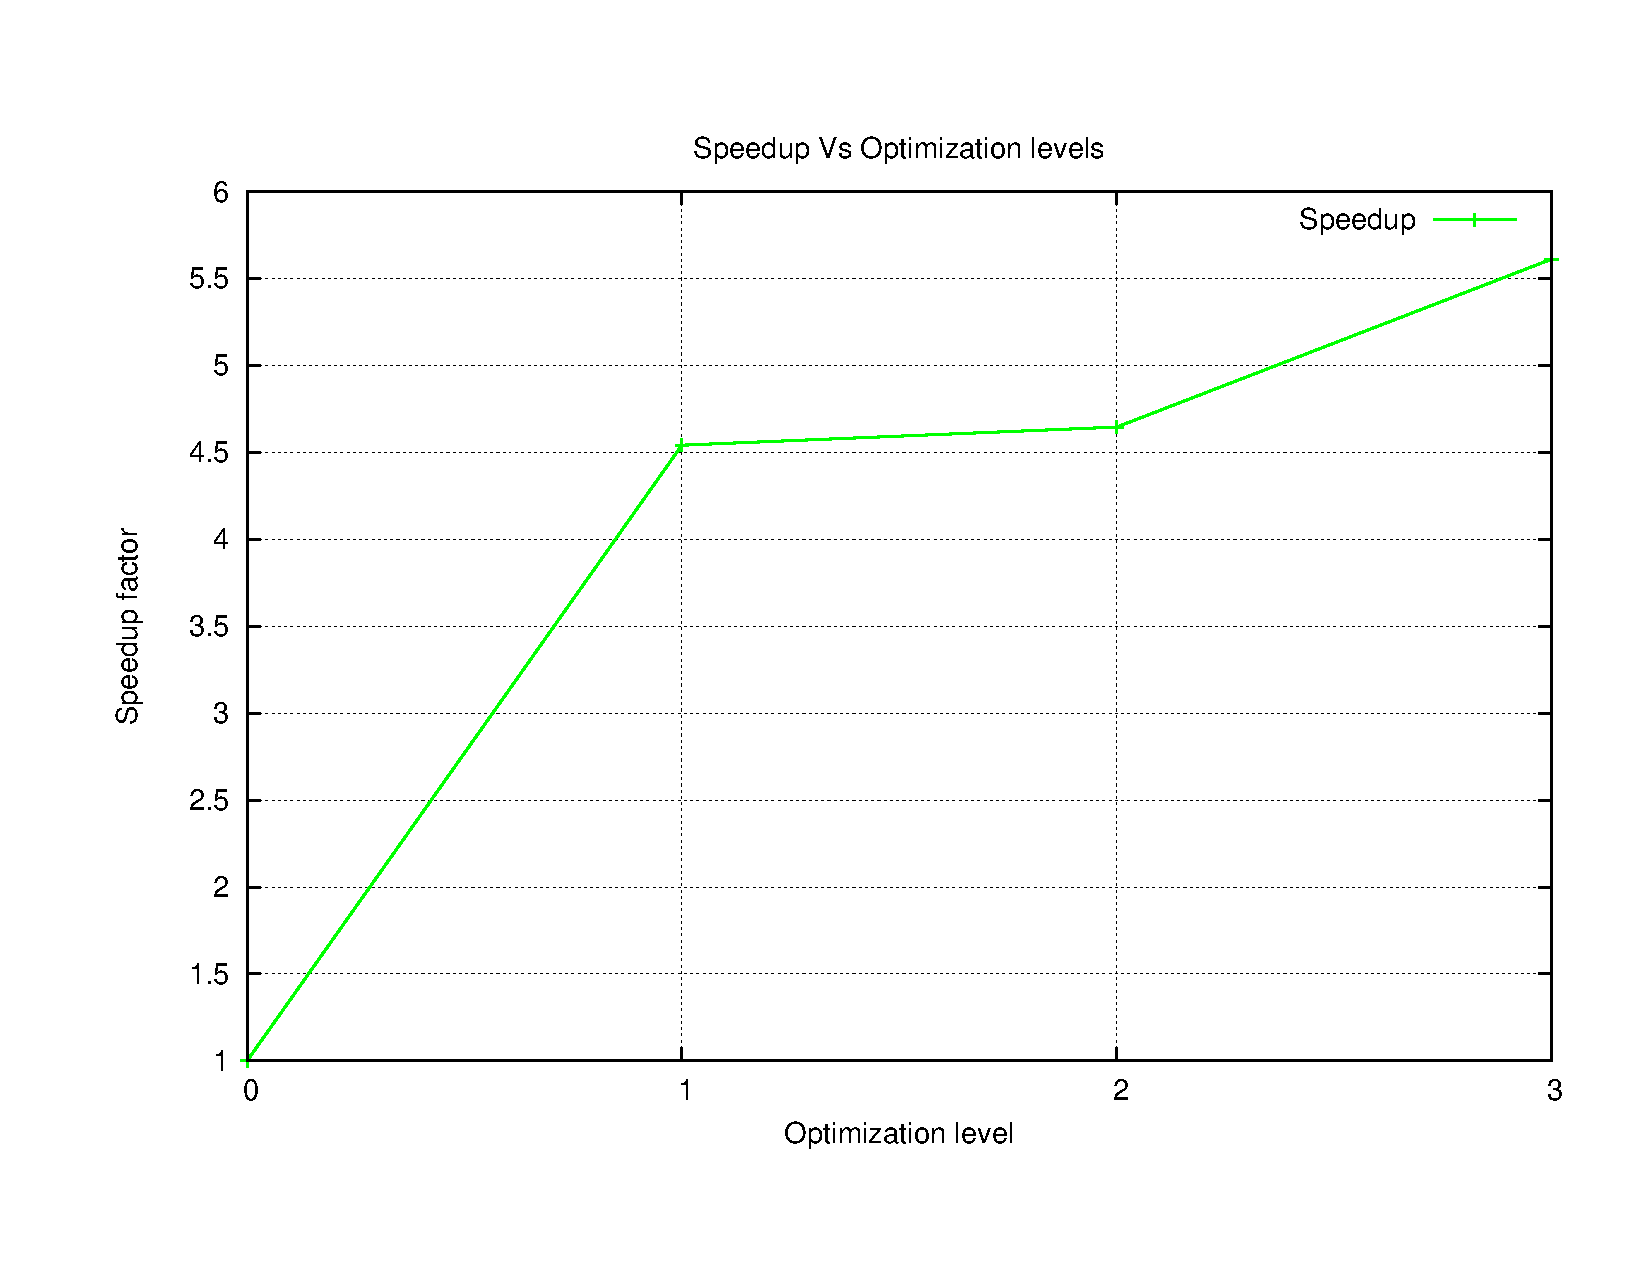
\includegraphics[trim=100 0 0 200,scale=0.22]{./Performance.pdf}
\end{figure}
\end{multicols}
\end{frame}

\section{Parallel Computing}
\begin{frame}{Parallelizing}
\begin{figure}[!htb]
\centering
\minipage{0.5\textwidth}
\centering
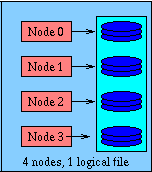
\includegraphics[scale=0.8]{./parallelio_0.png}

Parallel I/O 1 \cite{llnl}
\endminipage\hfill
\centering
\minipage{0.5\textwidth}
\centering
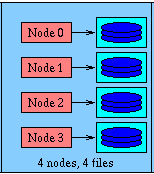
\includegraphics[scale=0.8]{./parallelio_1.png}

Parallel I/O 2 \cite{llnl}
\endminipage\hfill
\end{figure}
\end{frame}

\begin{frame}{Structure of Mesh files (Illustration)}
\begin{multicols}{2}
mxyz
\begin{tabular}{|c|c|}
\hline 
0	&	0	\\
0.5	&	0	\\
1	&	0	\\
\hline
2	&	0	\\
2	&	0.25	\\
2	&	0.5	\\
\hline
1.5	&	0.75	\\
1	&	0.75	\\
0.5	&	0.75	\\
\hline
0	&	0.5	\\
0	&	0.25	\\
0.5	&	0.25	\\
\hline 
\end{tabular} 

\columnbreak
mien
\begin{tabular}{|c|c|c|}
\hline					
8	&	11	&	10	 \\
9	&	2	&	8	 \\
1	&	4	&	7	 \\
\hline					
3	&	5	&	8	 \\
5	&	11	&	10	 \\
4	&	7	&	9	 \\
\hline					
6	&	8	&	3	 \\
10	&	3	&	9	 \\
7	&	1	&	2	 \\
\hline					
5	&	4	&	8	 \\
11	&	9	&	7	 \\
\hline
\end{tabular} 

\end{multicols}
\end{frame}

\begin{frame}[c]{First approach}
\begin{itemize}
\item  All the node information not present on indvidual processors. Mesh data needs to be communicated before the actual FEM code starts. This adds to communication overhead. 
\end{itemize}
\begin{figure}
\begin{picture}(0,0)
\put(25,85){$P0$}
\put(80,85){$P1$}
\put(135,85){$P2$}
\put(190,85){$P3$}
\end{picture}
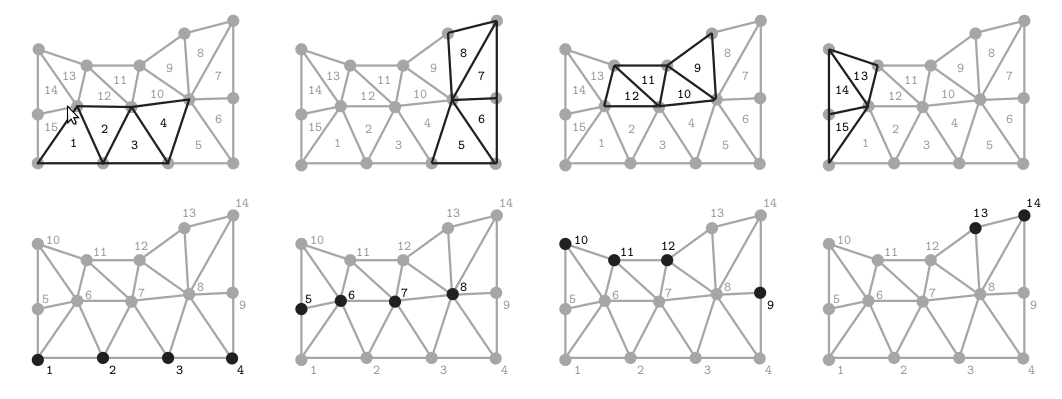
\includegraphics[scale=0.28]{./issue1.png}

Division of elements and nodes \cite{pccm}
\end{figure}
\end{frame}

\begin{frame}{Second approach}
\begin{itemize}
\item All mesh data present on the same processor. 
\end{itemize}
\begin{figure}[!htb]
\centering
\minipage{0.25\textwidth}
\centering
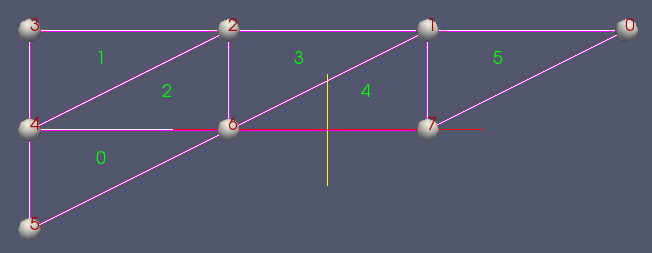
\includegraphics[scale=0.15]{./p0.png}

\textbf{P0}
\endminipage\hfill
\centering
\minipage{0.25\textwidth}
\centering
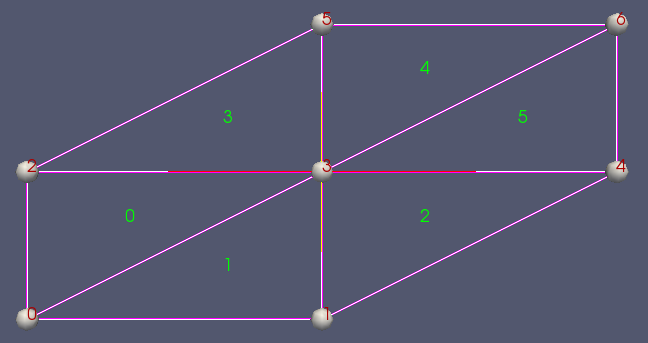
\includegraphics[scale=0.115]{./p1.png}

\textbf{P1}
\endminipage\hfill
\centering
\minipage{0.25\textwidth}
\centering
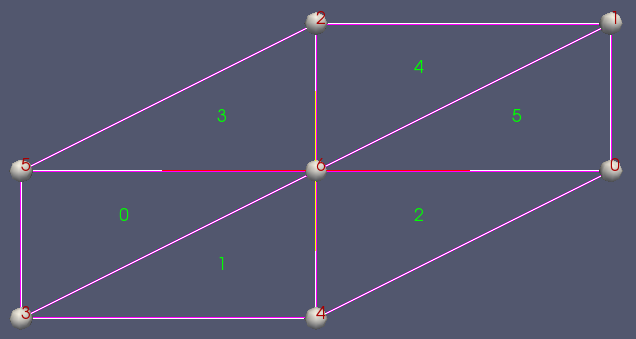
\includegraphics[scale=0.115]{./p2.png}

\textbf{P2}
\endminipage\hfill
\centering
\minipage{0.25\textwidth}
\centering
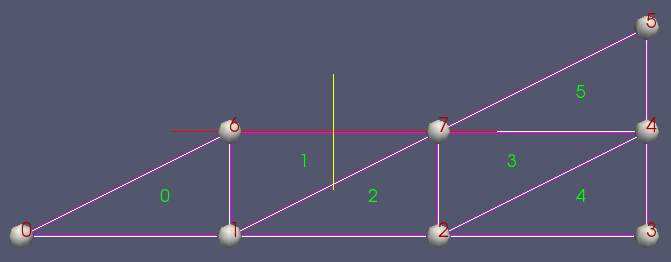
\includegraphics[scale=0.15]{./p3.png}

\textbf{P3}
\endminipage\hfill
\end{figure}
\begin{itemize}
\item A preprocessor is needed to generate the separate domains for each processor. Once the mesh is divided it can be reused in further simulations.
\end{itemize}
\end{frame}

\begin{frame}{Mesh Partitioning}
\begin{itemize}
\item Mesh partitioning tool needs to be used. 
\end{itemize}
\begin{figure}[!htb]
\centering
\minipage{0.5\textwidth}
\centering
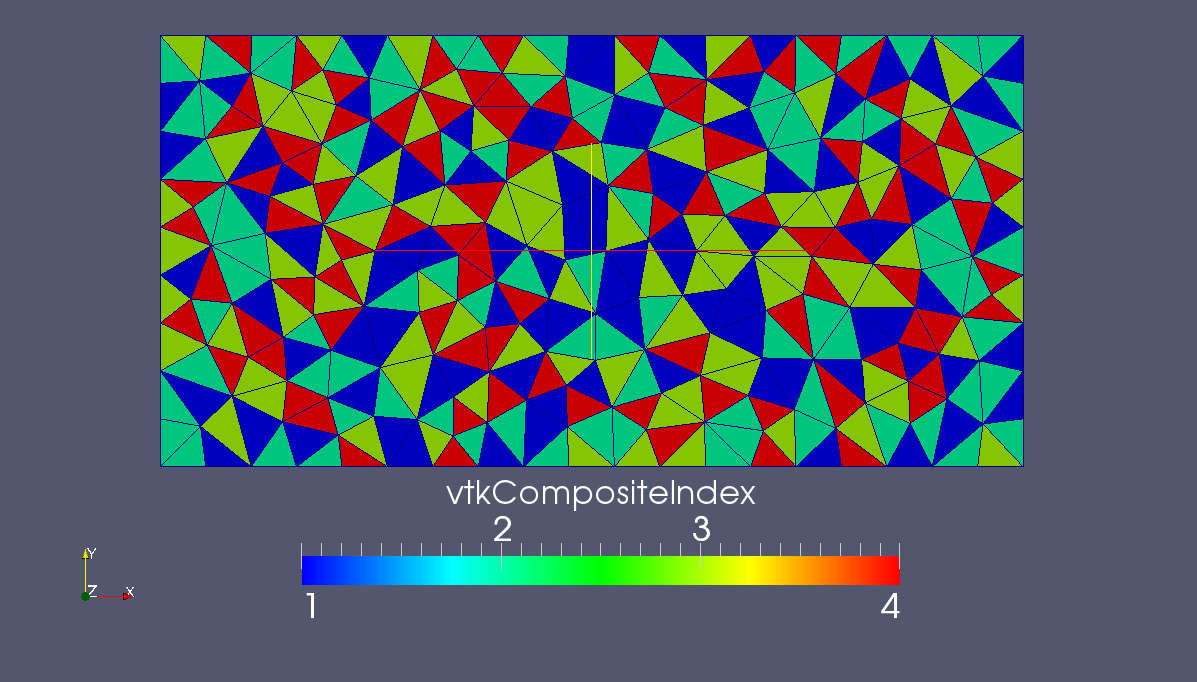
\includegraphics[scale=0.12]{./beforePartition.png}

Before Mesh partitioning
\endminipage\hfill
\centering
\minipage{0.5\textwidth}
\centering
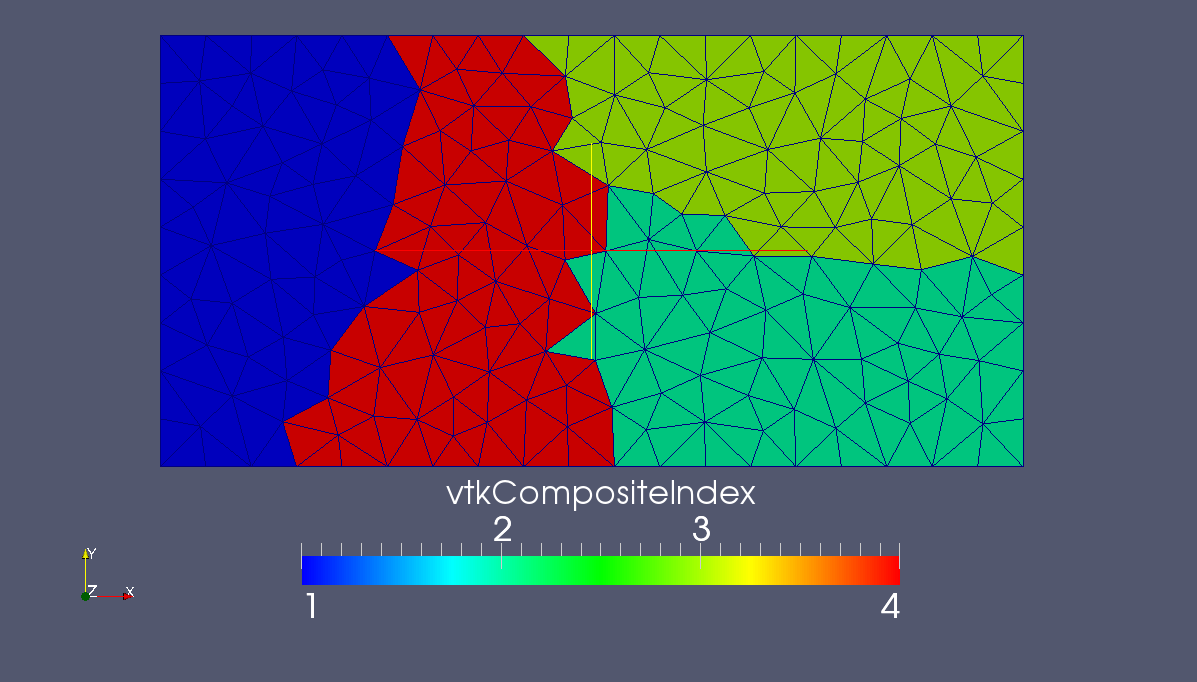
\includegraphics[scale=0.12]{./afterPartition.png}

After Mesh partitioning
\endminipage\hfill
\end{figure}
Several public tools available, e.g. SCOTCH, CHACO, HARP, JOSTLE, METIS, etc. We used METIS.
\end{frame}

\begin{frame}{Parallelizing with second approach}
\begin{multicols}{2}
\begin{figure}[!htb]
\centering
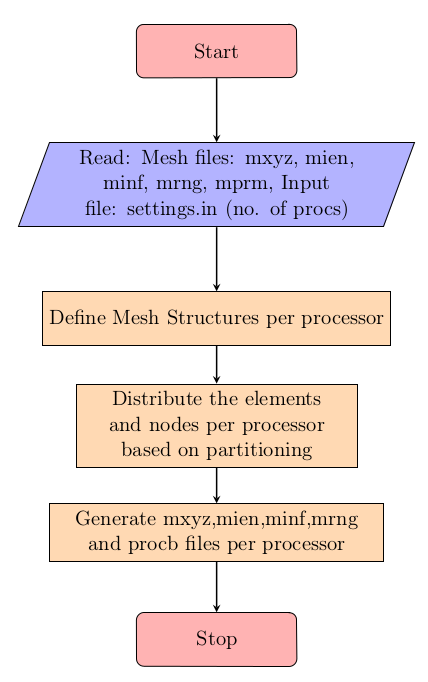
\includegraphics[trim=0 0 0 50,scale=0.3]{./preprocessorflowchart.png}

Preprocessor Flow Chart
\end{figure}

\columnbreak

 \text{Contents of a sample procb file}
\begin{center}
\begin{tabular}{cccccc}

0 & 0 & -1 & -1 & -1 & -1 \\ 

1 & 0 & -1 & -1 & -1 & -1 \\ 

2 & 0 & -1 & -1 & -1 & -1 \\ 

3 & 1 & 1 & -1 & -1 & -1 \\ 

13 & 1 & 1 & -1 & -1 & -1 \\ 

14 & 1 & 1 & -1 & -1 & -1 \\ 
 
15 & 2 & 1 & 2 & -1 & -1 \\ 
 
16 & 2 & 1 & 2 & -1 & -1 \\ 
\end{tabular} 
\end{center}

\end{multicols}
\end{frame}

\begin{frame}[c]{Program Flow Chart}
\begin{multicols}{2}
\begin{itemize}
\item[1]Preprocessing Stage:
	\begin{itemize}
	\item Reading settings and mesh data
	\end{itemize}
\item[2]Solution Stage:
	\begin{itemize}
	\item Calculating mesh metrics
	\item Applying boundary conditions
	\item Assembly of [M] and \{RHS\}
	\item Communicate [M] and \{RHS\} for boundary nodes
	\item Solve [M]\{T\} = \{RHS\}
	\end{itemize}
\item[3] Post Processing Stage
\end{itemize}
\columnbreak
\begin{figure}[ht!]
\centering
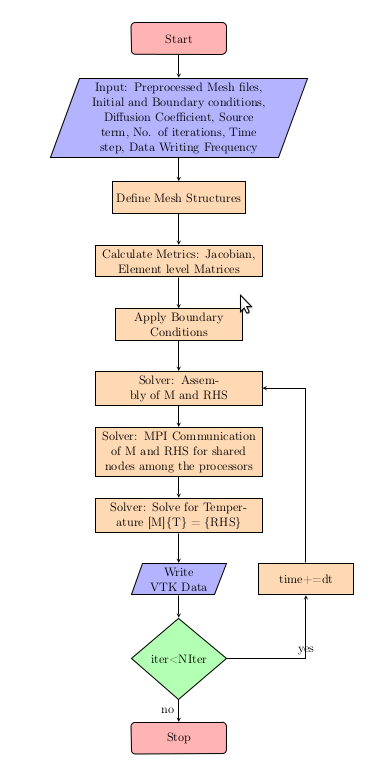
\includegraphics[trim=0 0 0 150,scale=0.4]{parallelflowchart1.png}
\end{figure}
\end{multicols}
\end{frame}

\begin{frame}{Verification of Parallel code}
A rectangular domain is considered for heat diffusion problem. Left and bottom walls are kept at 1000 K while top and right walls are maintained at 300 K and the temperature profile is allowed to develop over time. The snapshots are taken at t=0.001s, t=0.01s and t=0.1s.
\begin{figure}[!htb]
\centering
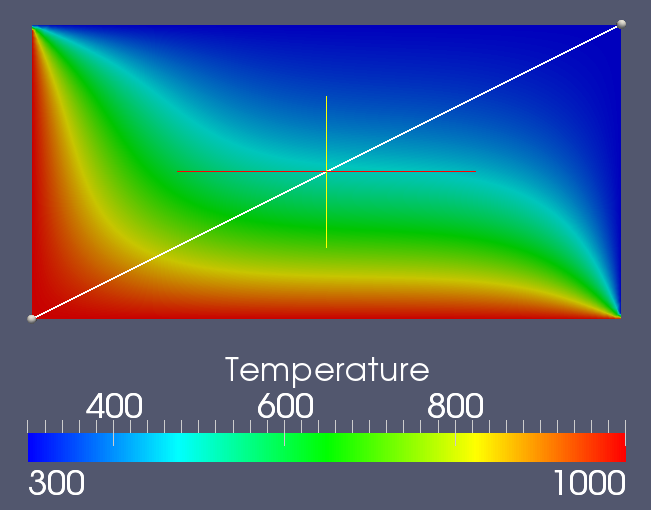
\includegraphics[trim=0 0 0 50,scale=0.22]{./verification_paraview.png}

t = 0.1 s
\end{figure}
\end{frame}

\begin{frame}{Verification of Parallel code}
\begin{figure}[!htb]
\centering
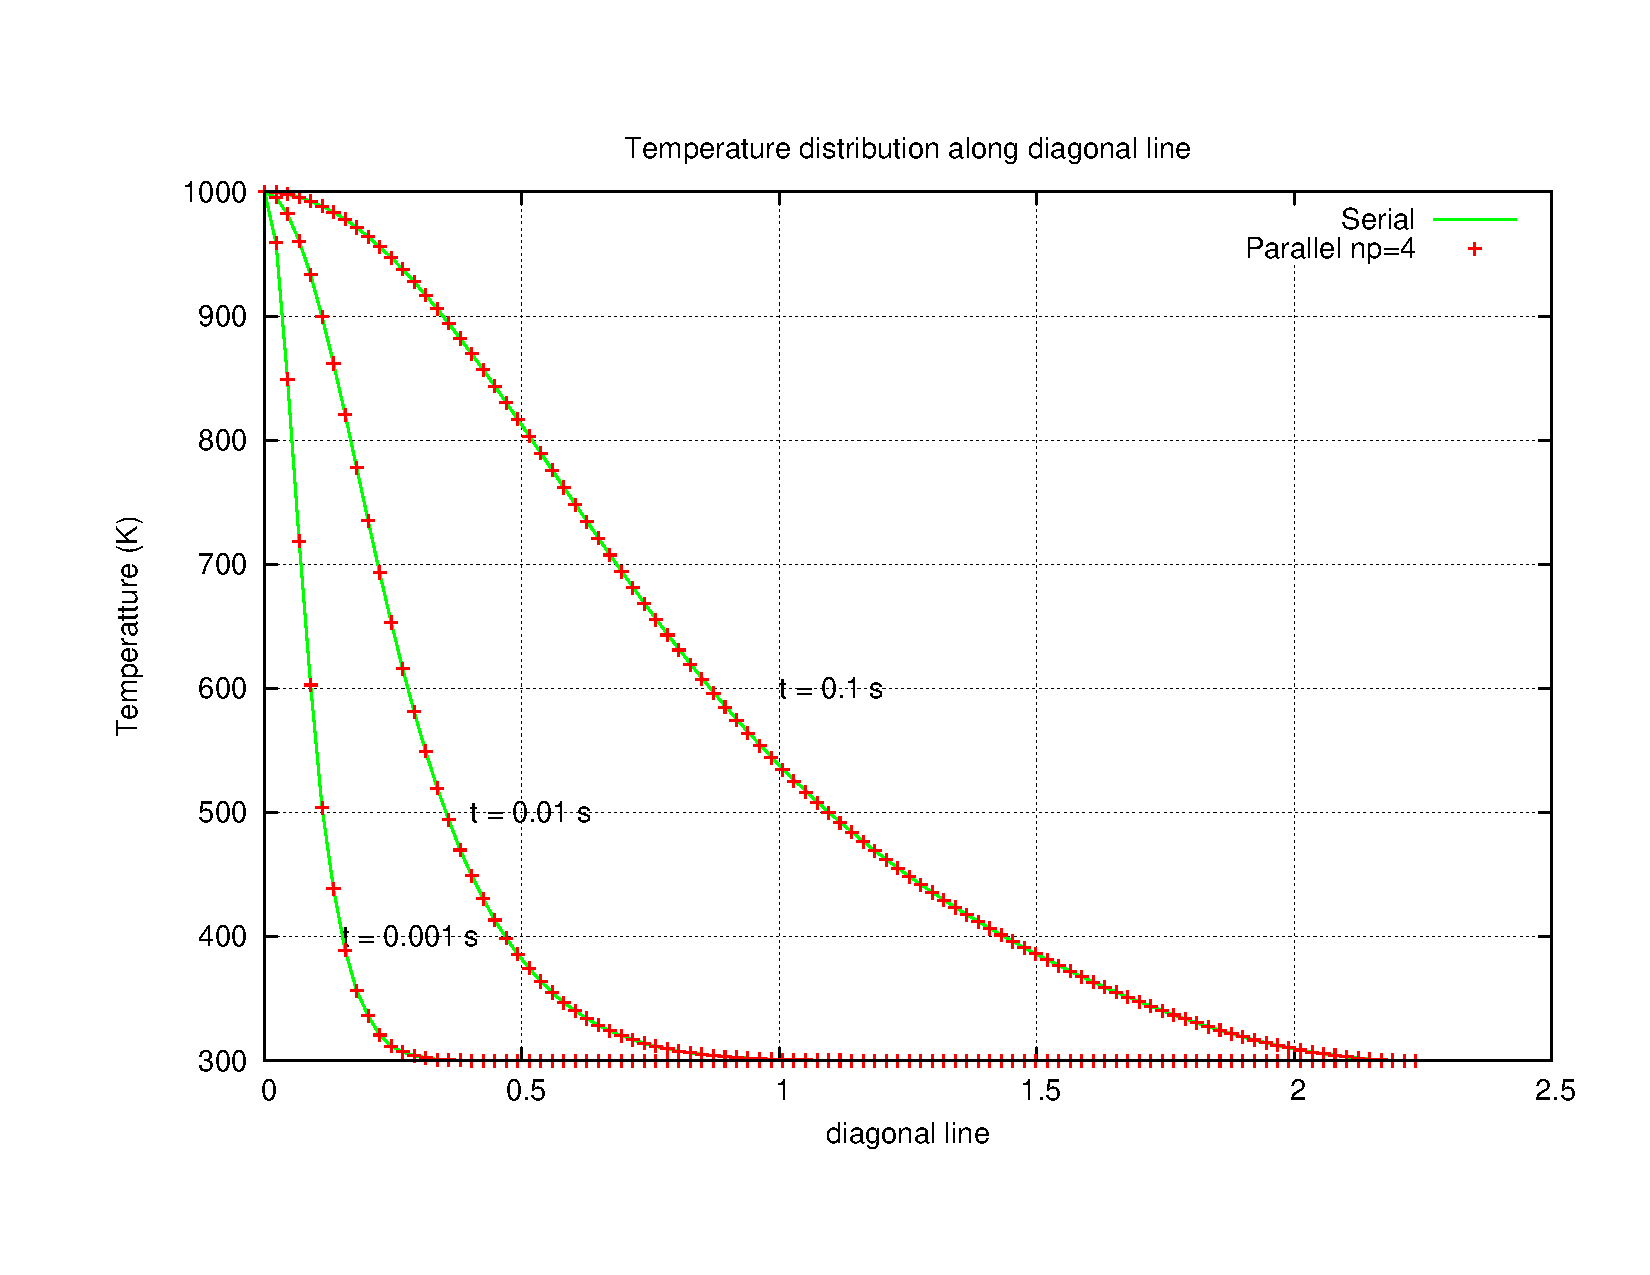
\includegraphics[trim=0 0 0 50,scale=0.3]{./verification_par.pdf}

\end{figure}
\end{frame}

\begin{frame}{Scalability}
\begin{figure}[!htb]
\centering
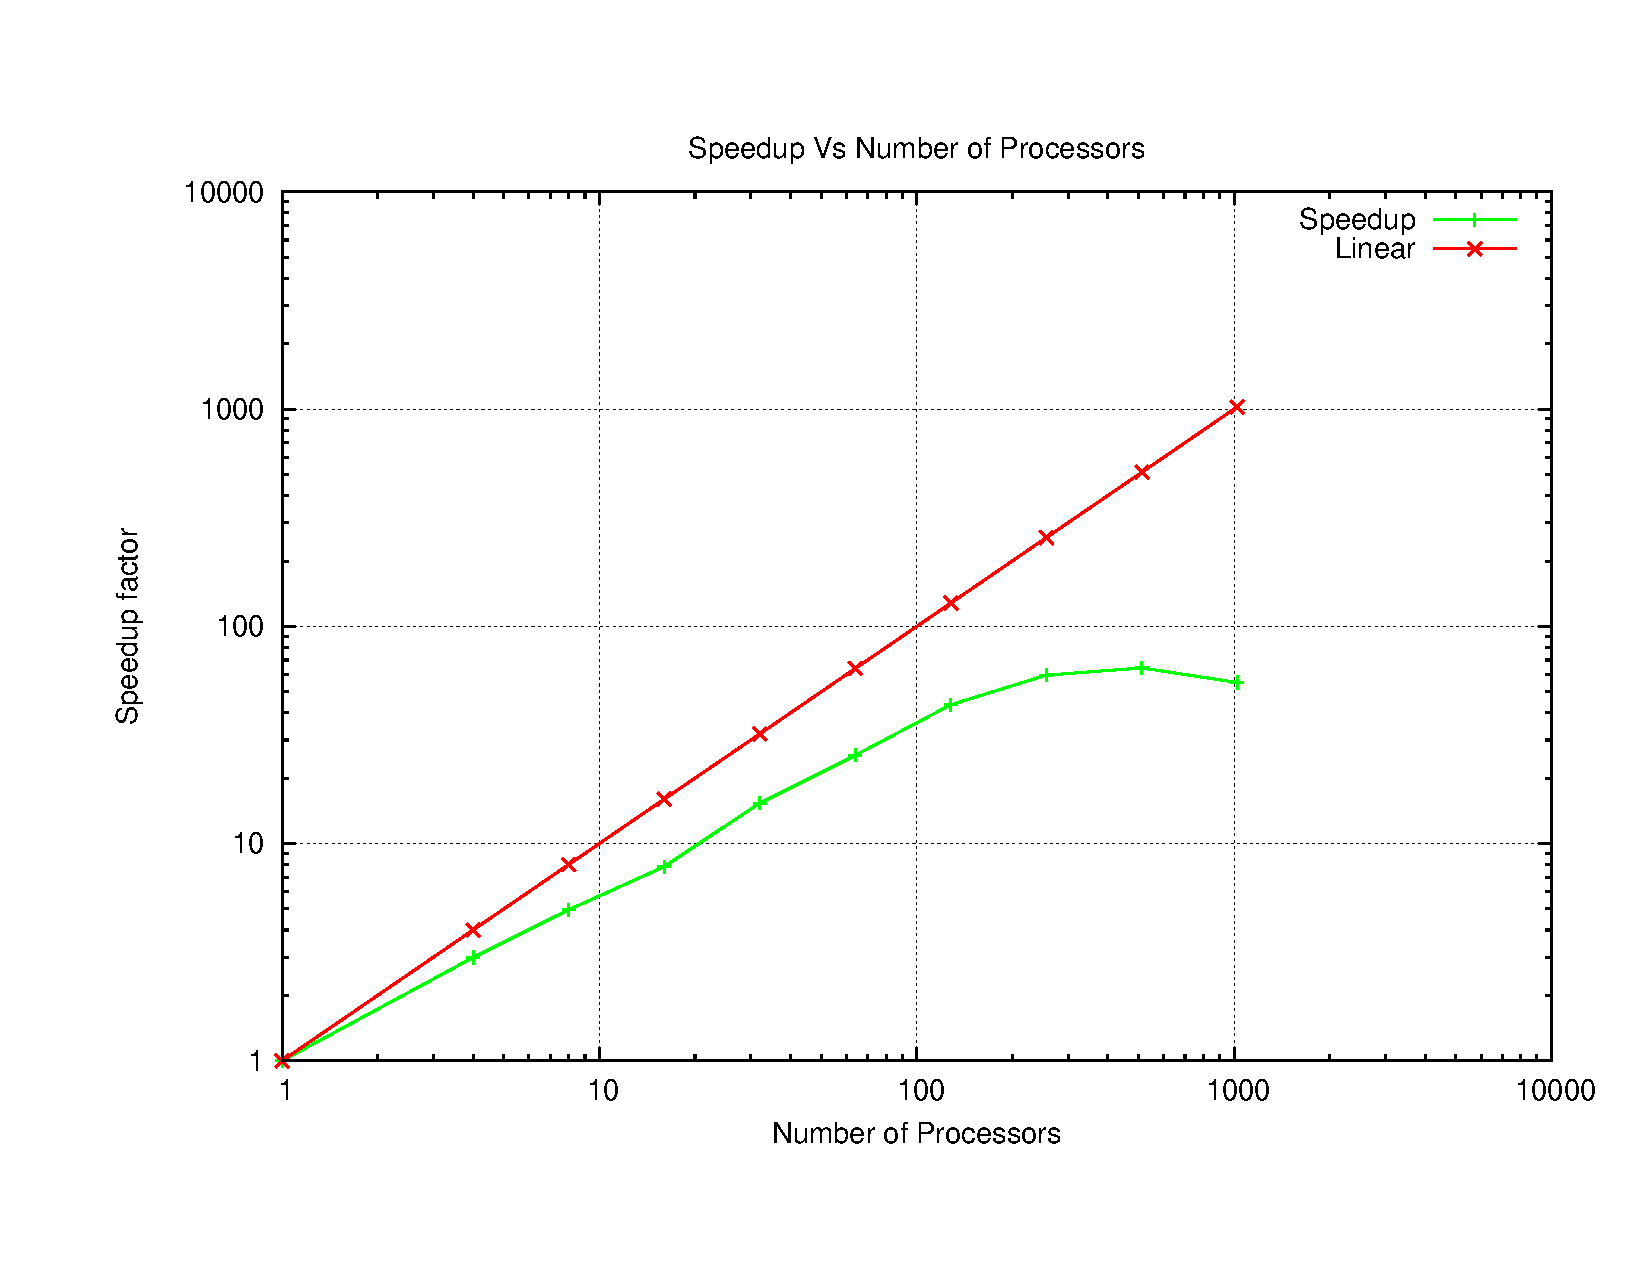
\includegraphics[trim=0 50 0 120,scale=0.3]{./Timings_1.pdf}

Finestmesh: ne = 516160, nn = 259082
\end{figure}
\end{frame}

\begin{frame}{Scalability [contd.]}
\begin{figure}[!htb]
\centering
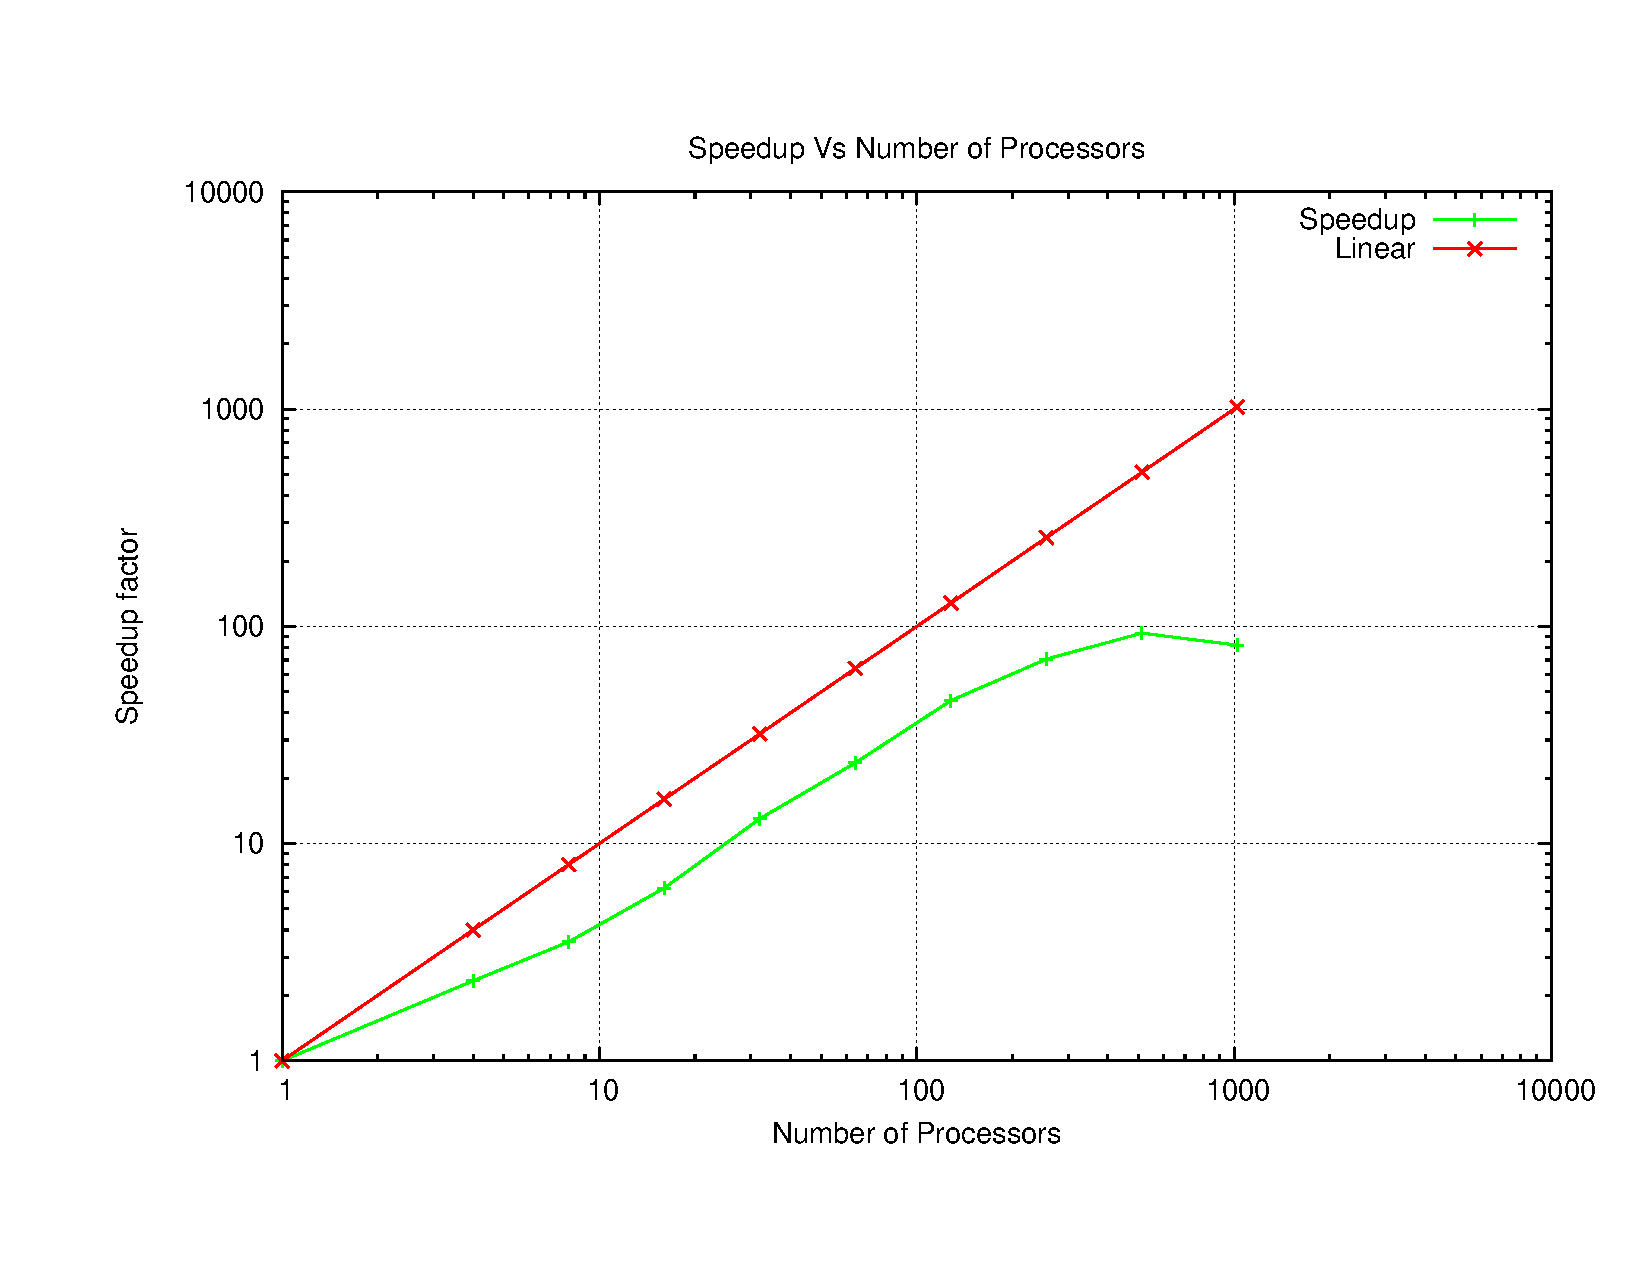
\includegraphics[trim=0 50 0 120,scale=0.3]{./Timings_2.pdf}

Superfine: ne = 945746, nn = 474074
\end{figure}
\end{frame}

\begin{frame}{Analysis using Scalasca}
\begin{figure}[!htb]
\centering
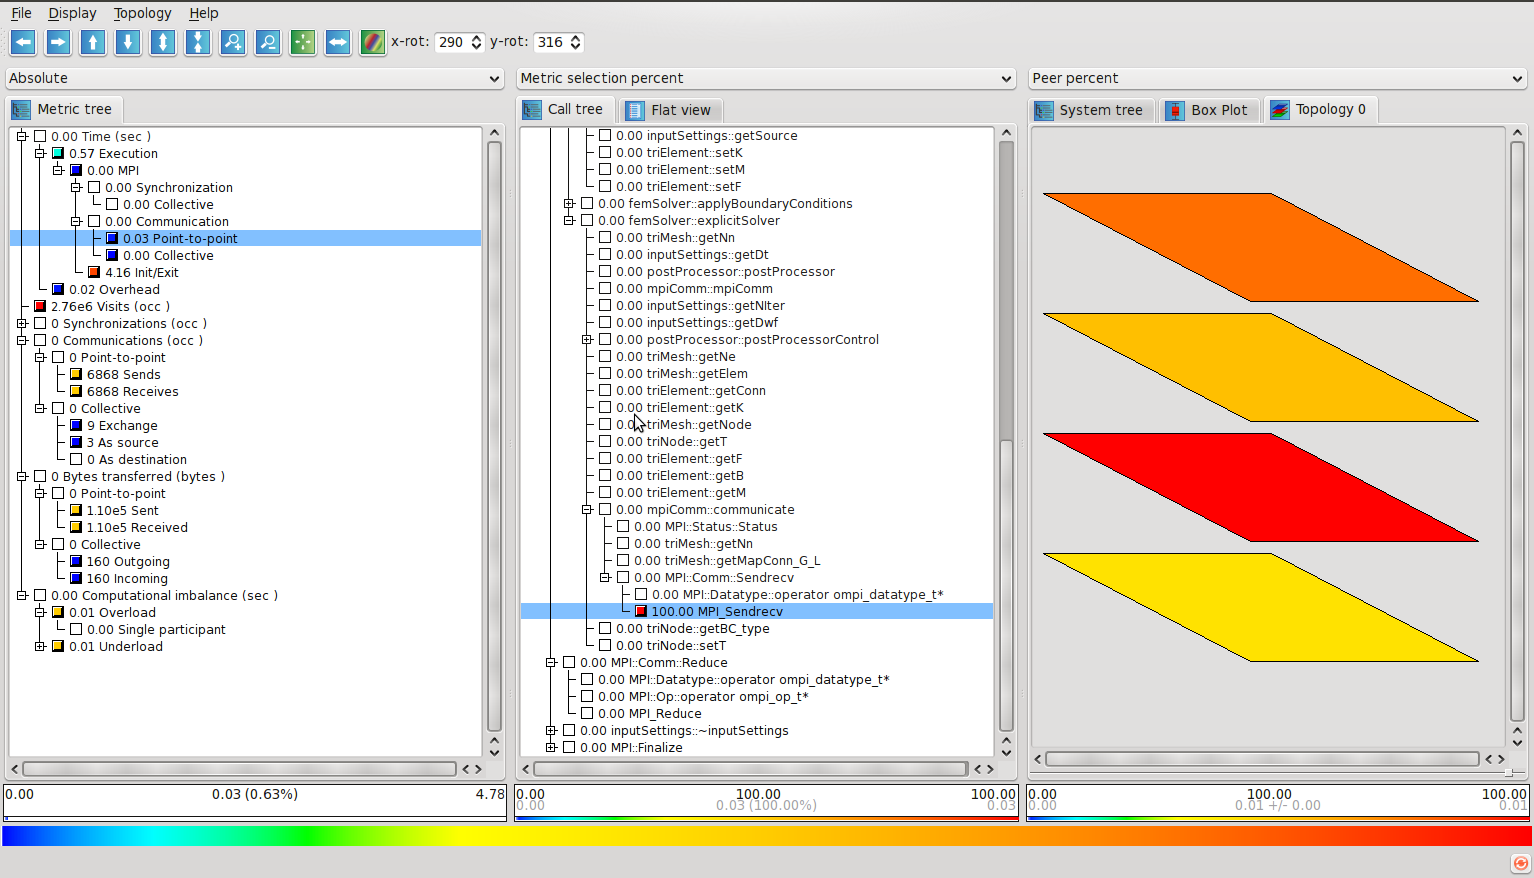
\includegraphics[trim=0 0 0 50,scale=0.25]{./scalasca.png}
\end{figure}
\end{frame}

\section{Application}
\begin{frame}{Application}
\begin{figure}[!htb]
\centering
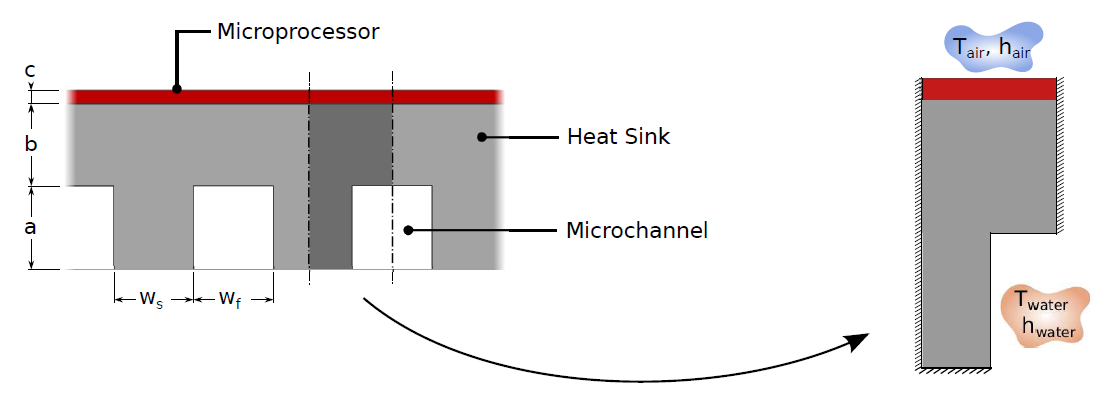
\includegraphics[scale=0.3]{./application.png}
\end{figure}
A heat sink for cooling computer chip, which is fabricated from copper with machined microchannels. Within these microchannels, water flows and carries away the heat dissipated by the chips. 
\end{frame}

\begin{frame}{Physical properties and dimensions:}
\begin{itemize}
\item Dimensions of the heat sink: 
a = b = $w_s$ = $w_f$ = 0.2 mm, c = 0.02 mm
\item Thermal diffusivity of copper: $\alpha_{copper}$ = 1.11 $\times$ $10^{-4}$ $m^2/s$
\item Density of copper: $\rho$ = 8940 $kg/m^3$
\item Specific heat capacity: $C_p$ = 385 J/kg/K
\item Properties of cooling fluid: $T_{water}$ = $25^o$ C, $h_{water}$ = 30000 $W/m^2/K$
\item Properties of ambient air: $T_{air}$ = $25^o$ C, $h_{air}$ = 2 $W/m^2/K$
\end{itemize}
\end{frame}

\begin{frame}
\begin{multicols}{2}
\textbf{Case 1:} Steady state temperature distribution 
\begin{figure}[!htb]
\centering
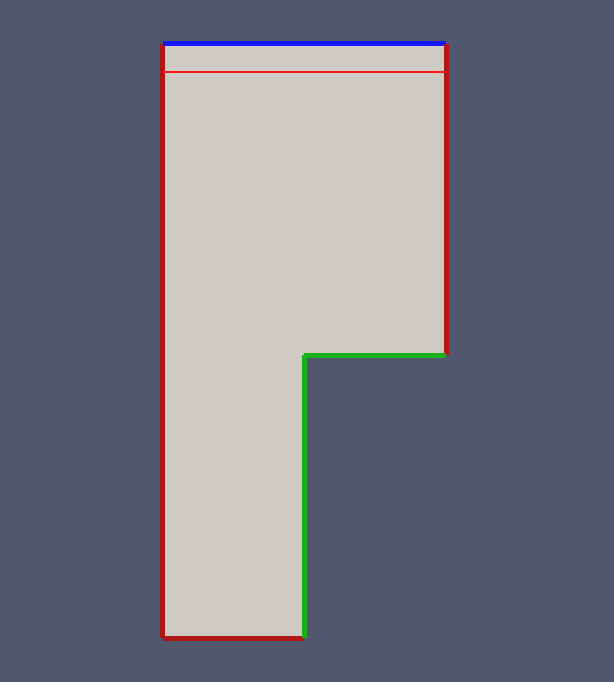
\includegraphics[trim=50 0 0 -30,scale=0.25]{./problem_def.png}
\begin{picture}(0,0)
\put(-110,60){{\small q=0}}
\put(-25,90){{\small q=0}}
\put(-80,0){{\small q=0}}
\put(-80,130){{\small $T_{wall}$=$75^o C$}}
\put(-55,35){{\small $T_{water}$=$25^o C$}}
\put(-25,115){{\small $\dot{q}$=0}}
\end{picture}
\end{figure}
%\begin{itemize}
%\item No heat generation
%\item Top surface temperature = $75^o$ C
%\item Determine temperature distribution in the domain
%\end{itemize}
\columnbreak
\textbf{Case 2}: Find $\dot{q}_{max}$ for $T_{max} < 75^0 C$
\begin{figure}[!htb]
\centering
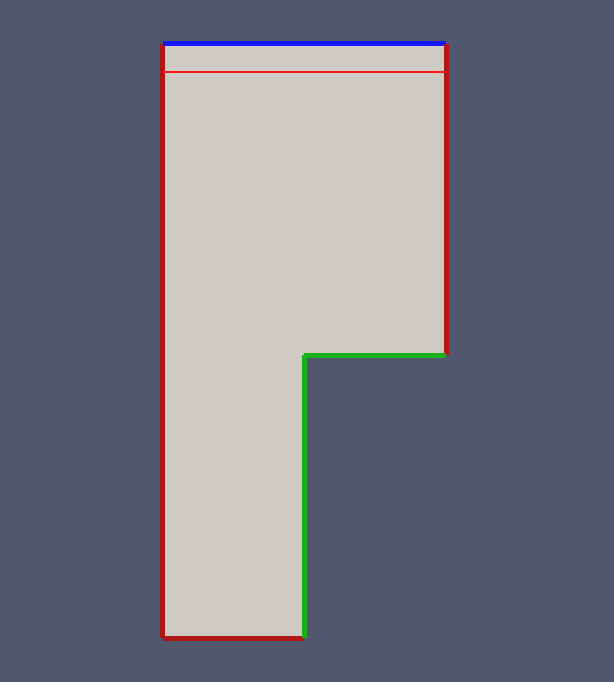
\includegraphics[trim=0 0 0 0,scale=0.25]{./problem_def.png}
\begin{picture}(0,0)
\put(-110,60){{\small q=0}}
\put(-25,90){{\small q=0}}
\put(-80,0){{\small q=0}}
\put(-80,130){{\small $T_{air}$=$25^o C$}}
\put(-55,35){{\small $T_{water}$=$25^o C$}}
\put(-25,115){{\small $\dot{q} \neq 0$}}
\end{picture}
\end{figure}
%\begin{itemize}
%\item Top surface exposed to ambient air
%\item Maximum allowed temperature in chip = $75^o$ C 
%\item Determine maximum heat generation allowed  for given condition
%\end{itemize}
\end{multicols}
\end{frame}

\begin{frame}{Case 1}
{\small Steady state criteria: Maximum rate of change of temperature in the domain $\left(\frac{dT}{dt}\right)_{max} \leq 0.001$}
\begin{figure}[!htb]
\centering
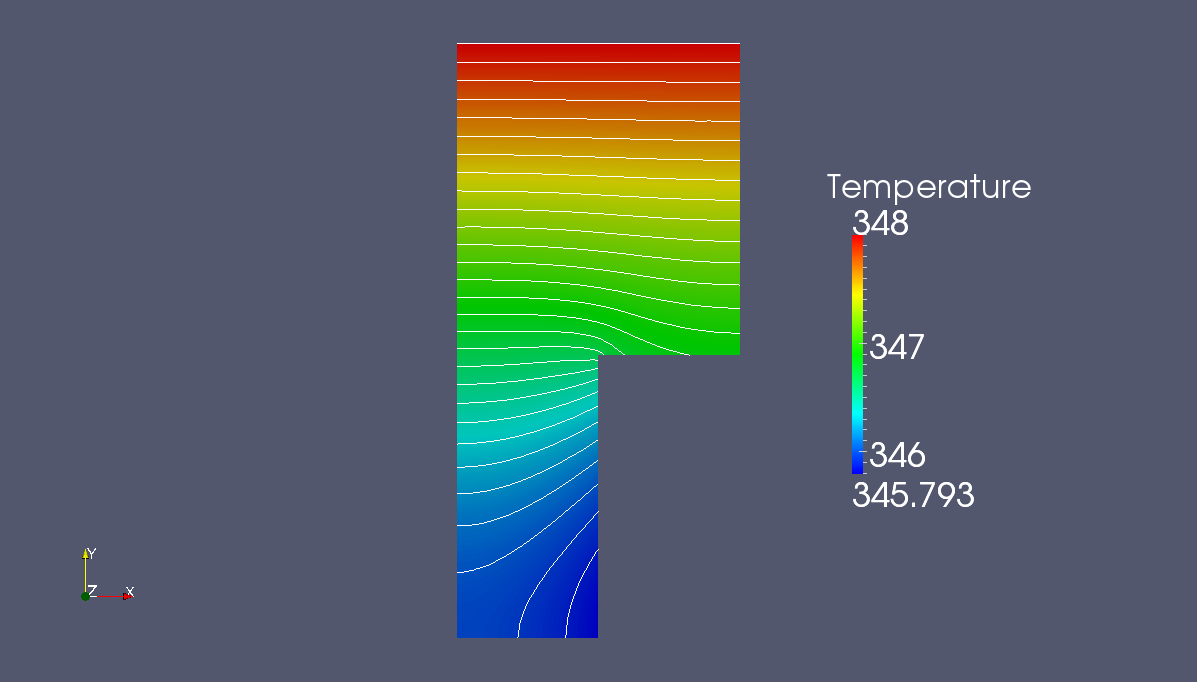
\includegraphics[scale=0.15]{./case1_c.png}
\end{figure}
Time required to reach steady state = \textbf{8.4237117 ms}
\end{frame}

\begin{frame}{Case 2}
{\small Use the result of case 1 as the initial condition. Maximum allowable temperature in the domain $75^o$C or 348 K}
\begin{figure}[!htb]
\centering
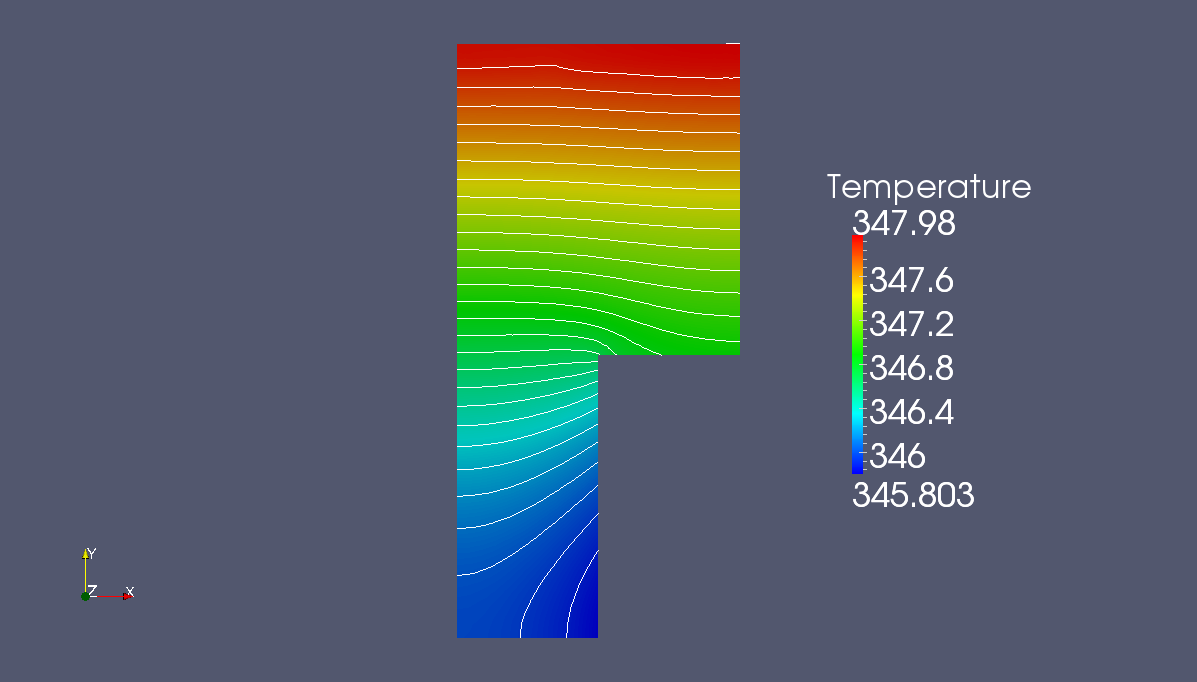
\includegraphics[trim=0 60 0 70,scale=0.15]{./case2_c.png}
\end{figure}
Maximum heat generation rate $\approx$ \textbf{9.6 $\times$ $10^{10}$ $W/m^3$}. 
If we consider a chip of dimensions $10$ mm$\times$10 mm $\times$ 0.02 mm, it is allowed to generate maximum \textbf{192 W}.
\end{frame}

\section{Summary}

\begin{frame}{Summary}
\begin{itemize}
\item A two dimensional transient heat diffusion equation is solved numerically using finite element method on unstructured mesh. 
\item A serial object oriented C++ code is developed based on the FE formulation.
\item The code is verified against analytical solutions found in \cite{jw}. 
\item The code is parallelized to be able to solve larger problems faster. 
\item The parallel code shows sufficient amount of scalability. 
\item Finally, the capability of the software to be applied to a realistic problem has been demonstrated.
\end{itemize}
\end{frame}

\begin{frame}[c]{References}
\bibliographystyle{unsrt}
\bibliography{ppt.bbl}
\end{frame}

\begin{frame}[c]

\begin{center}
{\Large Questions?}
\end{center}

\end{frame}
\end{document}
